\section{\textsc{Salatsauce mit Sahne und Dill}}

\subsection*{Zutaten für 300ml:}

\begin{tabular}{p{7.5cm} p{7.5cm}}
	& \\
	250ml saure Sahne oder Créme fraîche & 5g geschnittener Dill\\
	50ml Zitronen- oder Limettensaft & Salz \& Pfeffer
\end{tabular}

\subsection*{Serviervorschlag:}

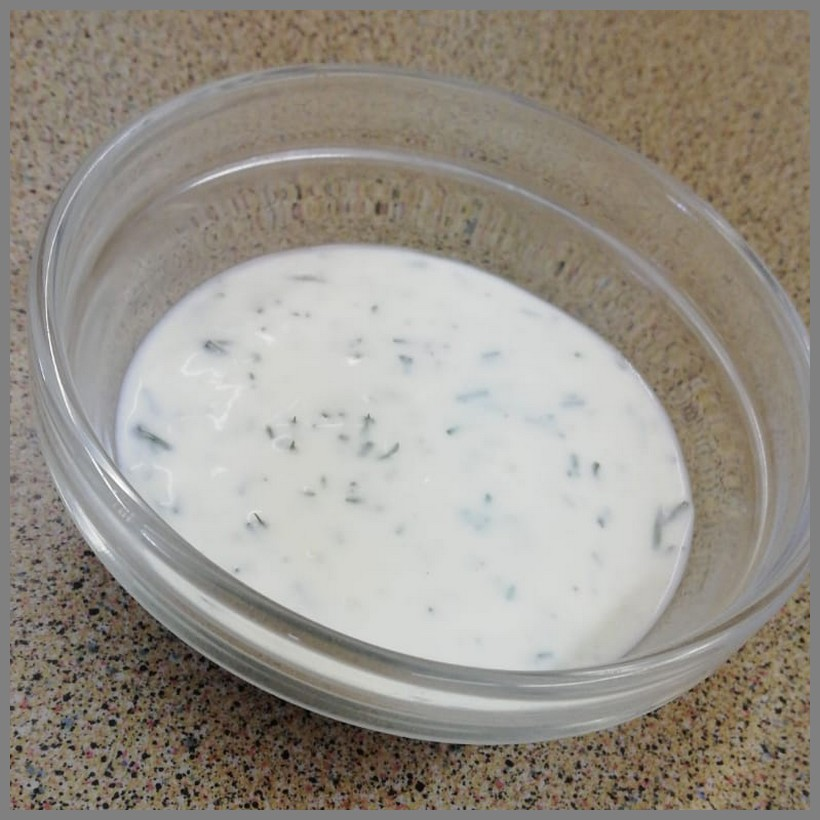
\includegraphics[width=\textwidth]{img/d_dillsahne.jpeg} \cite{dsahnedill}

\subsection*{So geht's:}

\begin{tabular}{p{15cm}}
	\\
	Sahne und Zitronensaft glattrühren.\\
	Dill dazugeben und mit Salz und Pfeffer abschmecken.\\
	\\
	Geeignet zu Blattsalat und Gemüsesalat.
\end{tabular}
